\chapter{Grundlagen und Stand der Forschung}
\label{StandDerForschung}
% VERSCHOBEN/ENTFERNT: Vorlagensatz "Dieses Kapitel ist normalerweise ..." entfernt

% GEÄNDERT: Kapiteleinleitung an die neue Reihenfolge angepasst (Systemübersicht zuerst, dann Verfahren, dann verwandte Arbeiten; Meeting-Notizen M3/M4). Der Satz "Beide Ausprägungen bilden gemeinsam den Untersuchungsgegenstand" wurde an den Umfang des Exposés angepasst (Customizing primär, Code kontextuell).
Zum Verständnis des in Kapitel~\ref{Ansatz} dargestellten Lösungsansatzes werden in diesem Kapitel zunächst die erforderlichen Grundlagen dargelegt, bevor die verwandten Arbeiten betrachtet werden, aus denen die Forschungslücke der vorliegenden Arbeit resultiert. Die Darstellung beschränkt sich dabei auf jene Begriffe sowie Verfahren, die für die Beantwortung der Forschungsfrage unmittelbar erforderlich sind, und gliedert sich in drei Teile. Der erste Teil stellt das betrachtete System vor, also den Aufbau eines SAP-Systems sowie die Stellen, an denen dessen individuelle Entwicklungen technisch hinterlegt sind. Den Schwerpunkt bilden dabei die Konfigurationsdaten, mit denen der generische Auslieferungsstandard an unternehmensspezifische Anforderungen angepasst wird, während die zusätzlich entwickelte Programmlogik nur so weit eingeführt wird, wie sie zur Erklärung dieser Konfiguration herangezogen wird. Der zweite Teil beschreibt die Verfahren, welche die methodische Grundlage des verfolgten Ansatzes bilden, also die semantische Interpretation durch ein Sprachmodell, die semantische Suche sowie den werkzeuggestützten Zugriff eines Agenten. Der dritte Teil ordnet die verwandten Arbeiten danach ein, wie nah sie der vorliegenden Problemstellung kommen und an welcher Stelle sie diese nicht mehr abdecken.

\section{Das betrachtete System}
\label{sec:system}

\subsection{ERP-Systeme und SAP S/4HANA}
\label{subsec:erp-s4}

\textbf{Betriebliche Standardsoftware und ERP-Systeme}
Betriebliche Standardsoftware bezeichnet vorgefertigte Anwendungssysteme, die
nicht für ein einzelnes Unternehmen individuell entwickelt, sondern als
generische Lösung für eine Vielzahl von Anwendern ausgeliefert werden. Ein
zentrales Beispiel bilden Enterprise-Resource-Planning-Systeme (ERP-Systeme),
die betriebswirtschaftliche Funktionsbereiche wie Rechnungswesen, Logistik sowie
Personalwirtschaft in einem integrierten System zusammenführen und dabei auf
einer gemeinsamen Datenbasis operieren \cite{klaus_what_2000}. Da ein solches
System die Prozesse zahlreicher Unternehmen unterstützen soll, bildet es zunächst
einen generischen Standard ab, der einen betriebswirtschaftlichen Referenzumfang
bereitstellt. Dieser Umfang wird im Zuge der Einführung an die spezifischen
Anforderungen des jeweiligen Unternehmens angepasst, wodurch sich
betriebsindividuelle Ausprägungen des ursprünglich einheitlichen Standards
ergeben.

Diese Anpassung ist regelmäßig erforderlich, sie erhöht jedoch zugleich den
Wartungsaufwand sowie die Komplexität des Systems, da sie die betriebliche
Prozesslogik zunehmend vom Herstellerstandard entkoppelt
\cite{light_maintenance_2001}. Über lange Betriebszeiträume hinweg verstärkt sich
dieser Effekt, sodass ein gewachsenes, schwer nachvollziehbares
Anpassungsportfolio entsteht, dessen unreflektierte Übernahme oder Beseitigung
mit erheblichen Risiken verbunden ist \cite{mhaskey_identifying_2025}. Dies
verdeutlicht, dass die Anpassung betrieblicher Standardsoftware ein grundlegendes
Spannungsfeld zwischen fachlicher Passgenauigkeit und technischer
Beherrschbarkeit begründet.

\textbf{Von der relationalen Datenbank zur In-Memory-Architektur}

Die klassischen SAP-Systemgenerationen R/3 sowie deren Nachfolger SAP ERP Central
Component (ECC) basieren auf einer dreischichtigen Client-Server-Architektur, die
Präsentations-, Applikations- sowie Datenbankebene voneinander trennt
\cite{buck-emden_technologie_1999}. Die Datenhaltung erfolgt dabei auf einer
zeilenorientierten relationalen Datenbank eines Drittanbieters, wobei
transaktionale Verarbeitung (OLTP) sowie analytische Auswertung (OLAP) aus
performancebedingten Gründen auf getrennten Systemen erfolgen: Da eine
zeilenorientierte Datenbank für lesende Aggregationen über große Datenmengen
ungeeignet ist, werden für Berichtszwecke zusätzliche, redundant vorgehaltene
Aggregatstabellen gepflegt \cite{plattner_common_2009}.

Mit SAP S/4HANA wird dieses Prinzip grundlegend verändert, indem die Anwendung
ausschließlich auf der spaltenorientierten In-Memory-Datenbank SAP HANA aufsetzt
\cite{sap_se_sap_nodate}. Die spaltenorientierte Speicherung sowie die
vollständige Vorhaltung der Daten im Arbeitsspeicher ermöglichen es,
transaktionale sowie analytische Workloads auf einer gemeinsamen Datenbasis zu
verarbeiten, wodurch die zuvor erforderlichen redundanten Aggregatstabellen
weitgehend entfallen \cite{plattner_common_2009, sikka_efficient_2012}. Dies
führt zugleich zu einer Vereinfachung des zugrunde liegenden Datenmodells, da
zahlreiche vormals zur Performancesteigerung notwendige Zusatzstrukturen im Zuge
der Umstellung entfernt werden. % NEU: Relevanzsatz ergänzt (Meeting-Notiz M2: stets erklären, warum ein Abschnitt für die FF wichtig ist)
Für die vorliegende Arbeit ist diese Entwicklung von Bedeutung, da die Überführung gewachsener Systeme auf SAP S/4HANA den in Abschnitt~\ref{sec:problem-ff} beschriebenen Analysebedarf auslöst.

\textbf{SAP S/4HANA als betrachtetes ERP-System}

Aufbauend auf dieser Betrachtung wird mit SAP S/4HANA das konkrete Produkt
beschrieben, in dessen Umfeld die Arbeit angesiedelt ist. Bei SAP S/4HANA handelt
es sich um das ERP-Kernprodukt der SAP~SE, das die zuvor beschriebenen, auf
relationalen Drittanbieter-Datenbanken basierenden Systemgenerationen ablöst
\cite{gerard_sap_2017}. Für die vorliegende Arbeit sind zwei Eigenschaften der
Anwendungsschicht besonders relevant. Zum einen werden sämtliche Datenstrukturen
zentral im Data Dictionary (DDIC) verwaltet, das die Definitionen aller Tabellen,
Felder und Datentypen systemweit vorhält und damit die Grundlage für eine
metadatenbasierte Analyse bildet. Zum anderen ist ein SAP-System
mandantenfähig, das heißt, es kann mehrere voneinander abgeschottete
Datenbestände (Mandanten) innerhalb einer Installation führen, was bei der
Auswahl und Interpretation von Customizing-Daten zu berücksichtigen ist.

% GEÄNDERT: bisherige TikZ-Grafik durch externe, bearbeitbare draw.io-Grafik ersetzt, die zusätzlich zeigt, wo Customizing und Eigenentwicklungen liegen (Meeting-Notiz M3 "Systemübersicht"; Grafik G2). Die TikZ-Datei bleibt im Ordner Grafiken erhalten.
Abbildung~\ref{fig:systemuebersicht} zeigt den Aufbau eines solchen Systems und hebt hervor, an welchen Stellen die für diese Arbeit relevanten Objekte liegen.

\begin{figure}[htbp]
	\centering
	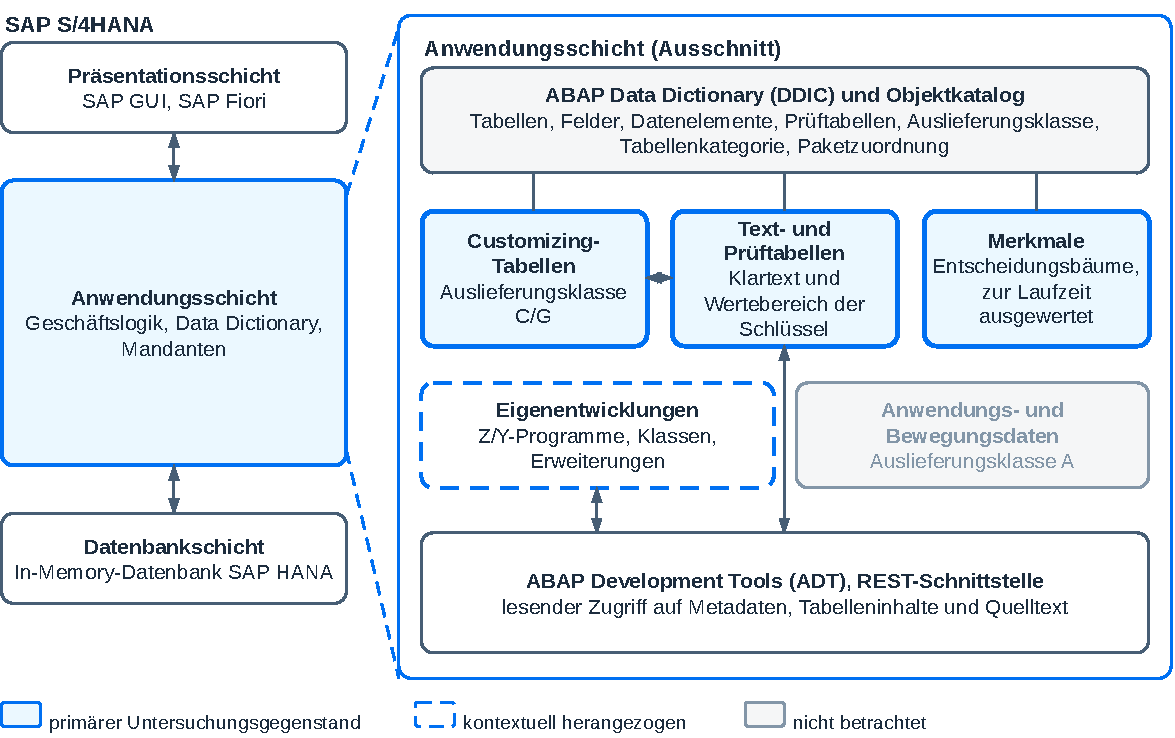
\includegraphics[width=\linewidth]{Grafiken/abb2_1_systemuebersicht.pdf}
	\caption{Aufbau eines SAP-S/4HANA-Systems und Lage der individuellen Entwicklungen in der Anwendungsschicht (eigene Darstellung in Anlehnung an \cite{buck-emden_technologie_1999, gerard_sap_2017}).}
	\label{fig:systemuebersicht}
\end{figure}

\subsection{Customizing, Eigenentwicklung und Abweichung vom Standard}
\label{subsec:customizing}

Die Anpassung eines solchen Systems reicht von der reinen Konfiguration
bestehender Funktionalität bis zur Programmierung zusätzlicher Anwendungslogik
\cite{brehm_tailoring_2001}. Für die vorliegende Arbeit wird diese
Bandbreite auf zwei Pole zugespitzt, deren Unterscheidung für den weiteren
Verlauf zentral ist: das Customizing im engeren Sinne als tabellengesteuerte
Konfiguration sowie die Eigenentwicklung als zusätzlich programmierte Anwendungslogik.

% NEU: Einführung von Auslieferungsklasse und Tabellenkategorie (aus Textbaustein 11.09.2026), da der Entwurf in 3.4.1 darauf aufbaut
\textbf{Auslieferungsklasse und Tabellenkategorie}

Das DDIC beschreibt eine Tabelle nicht allein über ihre Felder, sondern führt zu jeder Tabelle zusätzlich zwei Merkmale, die deren Rolle im System festlegen. Die Auslieferungsklasse bestimmt, wie eine Tabelle bei Auslieferung sowie beim Transport zwischen Systemen behandelt wird, und unterscheidet dabei insbesondere Anwendungsdaten von Customizing-Daten. Die Tabellenkategorie legt demgegenüber fest, ob es sich um eine transparente, in der Datenbank physisch angelegte Tabelle oder um eine ausschließlich im Programmkontext verwendete Struktur handelt \cite{sap_ddic_delivery_class}. Beide Merkmale sind für jedes Objekt gepflegt sowie maschinell auswertbar und ordnen ein Objekt damit unabhängig von seiner sprachlichen Beschreibung einer Objektklasse zu. Dies ist für den vorliegenden Ansatz von Bedeutung, da sich auf diesem Weg deterministisch bestimmen lässt, ob eine Tabelle Customizing trägt.

% NEU: Schlüssel-, Text- und Prüftabellen sowie Merkmale am durchgängigen Beispiel (Meeting-Notiz M11)
\textbf{Schlüsselwerte, Text- und Prüftabellen sowie Merkmale}

Customizing-Tabellen speichern ihre Inhalte überwiegend als kurze Schlüsselwerte, deren fachliche Bedeutung nicht in derselben Tabelle hinterlegt ist. Der zulässige Wertebereich eines Feldes wird über eine Prüftabelle festgelegt, die im DDIC als Fremdschlüsselbeziehung gepflegt ist, während der zugehörige sprachabhängige Klartext in einer Texttabelle abgelegt ist. Eine lesbare Aussage über eine Konfiguration setzt folglich voraus, dass diese Beziehungen verfolgt werden. Hinzu kommen im Personalwesen sogenannte Merkmale, die einen Wert nicht fest hinterlegen, sondern ihn zur Laufzeit über einen gepflegten Entscheidungsbaum aus Eigenschaften eines Beschäftigten ermitteln. Im durchgängigen Beispiel ordnet ein solches Merkmal die Gruppe der Auszubildenden einer Regelgruppe zu, eine Customizing-Tabelle legt je Regelgruppe die beantragbaren Abwesenheitsarten als Schlüsselwerte fest, und erst eine Texttabelle liefert deren Bezeichnungen. % [BELEG ERFORDERLICH: Merkmale (T549B/T549C) im SAP-Personalwesen, z. B. SAP-Hilfe zum Merkmal WEBMO]
% Hinweis: Tabellenkette laut Testfall TC1-S3 (tests/cases.py): T549C -> T554S_WEB -> T554T; T554T dort als "hyp" markiert, vor Nennung im Text am System bestätigen.

\textbf{SAP-Standard, Abweichung und Standardnähe}

Aus der Unterscheidung zwischen dem ausgelieferten Standard und der
betriebsindividuellen Anpassung ergibt sich der für diese Arbeit zentrale Begriff
der Abweichung vom SAP-Standard. Eine Abweichung bezeichnet jede Ausprägung eines
Systems, die vom Auslieferungszustand des Herstellers abweicht, sei es durch
veränderte Konfigurationswerte im Customizing oder durch zusätzliche
Eigenentwicklungen. Das Ausmaß, in dem ein System dem Auslieferungszustand
entspricht, wird als Standardnähe bezeichnet und lässt sich kennzahlenbasiert
quantifizieren \cite{sekatzek_messung_2009}. Ein methodisch verwandter Zugang
besteht darin, aus einem produktiv eingesetzten System ein Modell der tatsächlich
genutzten sowie angepassten Elemente abzuleiten \cite{nuttgens_reverse_1999}.
Beide Zugänge bestimmen jedoch primär das Vorhandensein sowie den Grad einer
Abweichung, während deren fachliche Bedeutung unberücksichtigt bleibt; ebendiese
Deutung bildet den Ausgangspunkt der vorliegenden Arbeit und wird in Abschnitt~\ref{sec:stand-forschung} vertieft betrachtet. % GEÄNDERT: Verweis präzisiert
Die Frage, gegen welche Referenz eine Abweichung im Einzelfall bestimmt wird, ist damit noch nicht beantwortet und wird als Teil des Entwurfs in Abschnitt~\ref{subsec:ta-abweichung} behandelt. % NEU: Vorverweis auf die Operationalisierung

\subsection{Technischer Zugang über Data Dictionary und ADT}
\label{subsec:zugang}

Die Analyse einer solchen Abweichung setzt einen technischen Zugang zu den
beschriebenen Materialien voraus. Das bereits eingeführte Data Dictionary (DDIC)
enthält die Metadaten sowohl der Standard- als auch der kundeneigenen Objekte und
bildet damit den zentralen Ansatzpunkt dieses Zugangs. Der lesende Zugriff auf
Quelltexte, Tabelleninhalte sowie Objektmetadaten ist über die ABAP Development
Tools (ADT) möglich, die hierfür eine auf dem HTTP-Protokoll basierende
Schnittstelle bereitstellen. Diese Schnittstelle bildet die technische Grundlage,
über die der in dieser Arbeit entwickelte Ansatz die relevanten
Systeminformationen erschließt.

% GEÄNDERT: Überleitung an die neue Gliederung angepasst
Die in diesem Abschnitt eingeführten Objekte bilden damit den Gegenstand der Untersuchung. Im folgenden Abschnitt werden die Verfahren dargelegt, mit denen diese Objekte erschlossen, interpretiert sowie gegen den Systemzustand abgesichert werden.

\section{Grundlagen der Verfahren}
\label{sec:verfahren}
% GEÄNDERT: Überschrift korrigiert; der bisherige Abschnitt "Stand der Forschung" enthielt Verfahrensgrundlagen und keine verwandten Arbeiten

% GEÄNDERT: Satzfragment "Ergänzt durch Verfahren ..." aufgelöst; Schema-Linking und Verifikation werden nun in 2.3 als verwandte Arbeiten behandelt
Aufbauend auf dem zuvor beschriebenen System werden im Folgenden die Verfahren dargelegt, die das methodische Fundament des verfolgten Ansatzes bilden. Diese reichen von den Sprachmodellen als interpretierende Instanz über deren Verankerung an überprüfbaren Quellen sowie die semantische Suche bis zu der Schnittstelle, über die ein modellgesteuerter Agent selbstständig auf das System zugreift.

\subsection{Sprachmodelle, Grounding und Retrieval-Augmented Generation}
\label{subsec:llm-grounding}

\textbf{Large Language Models}
Große Sprachmodelle (Large Language Models, LLMs) sind neuronale Netze, die auf umfangreichen Datensätzen trainiert werden und darauf ausgelegt sind, natürlichsprachliche Eingaben zu verarbeiten sowie fortzusetzen \cite{zhao_survey_2026}. Viele moderne LLMs basieren auf der Transformer-Architektur, deren Self-Attention-Mechanismus es ermöglicht, Abhängigkeiten zwischen unterschiedlichen Positionen einer Eingabesequenz direkt zu modellieren \cite{vaswani_attention_2017}. Eine für die vorliegende Arbeit wesentliche Eigenschaft besteht darin, dass hinreichend große Modelle Aufgaben allein anhand weniger Beispiele oder einer natürlichsprachlichen Anweisung im Eingabekontext bewältigen können, ohne dass ein erneutes Training erforderlich ist \cite{brown_language_2020}. Dies erlaubt es, ein Modell über die Gestaltung der Eingabe (Prompt) für eine spezifische Aufgabe zu steuern.
Dieser Steuerbarkeit stehen jedoch Einschränkungen gegenüber, die für den Einsatz in einem fachlich sensiblen Kontext berücksichtigt werden müssen. Zum einen neigen LLMs dazu, inhaltlich falsche, aber sprachlich plausible Aussagen zu erzeugen, ein Phänomen, das als Halluzination bezeichnet wird \cite{gao_retrieval-augmented_2024}. Besonders problematisch ist, dass ein Modell in produktiven Datenbeständen nicht offen scheitert, sondern mit hoher Überzeugung. Es erzeugt syntaktisch gültige, plausibel wirkende Abfragen, die auf die falschen Objekte verweisen, und liefert ein Ergebnis, ohne dass dessen Unzuverlässigkeit erkennbar wäre \cite{helwig_metadata_2026}. Zum anderen ist die Menge an Information, die ein Modell gleichzeitig verarbeiten kann, durch die Größe des Kontextfensters begrenzt, sodass umfangreiche Artefakte nicht vollständig übergeben werden können. Diese Einschränkungen begründen den Bedarf, dem Modell die benötigten fachlichen Informationen gezielt sowie belegbar bereitzustellen, anstatt sich auf dessen internes, aus dem Training stammendes Wissen zu verlassen.

\textbf{Grounding und Retrieval-Augmented Generation}
Als Grounding wird die Verankerung der Modellausgabe in überprüfbaren, externen Informationsquellen bezeichnet, mit der den zuvor genannten Einschränkungen begegnet wird. Ein etabliertes Verfahren hierfür ist die Retrieval-Augmented Generation (RAG), bei der relevante Informationen zunächst aus einer externen Wissensquelle abgerufen und anschließend gemeinsam mit der eigentlichen Anfrage an das Modell übergeben werden \cite{lewis_retrieval-augmented_2021}. Dadurch wird die Ausgabe an die bereitgestellten Inhalte gebunden, wodurch sich sowohl die faktische Genauigkeit erhöht als auch die Nachvollziehbarkeit der Aussagen verbessert \cite{gao_retrieval-augmented_2024}. Dieses Prinzip ist für die vorliegende Arbeit von besonderer Bedeutung, da die fachliche Bedeutung eines Customizing-Befunds nicht dem allgemeinen Trainingswissen des Modells entnommen, sondern aus dem konkreten Systemzustand sowie zugehörigen Wissensquellen abgeleitet werden muss.

\subsection{Semantische Suche über Text-Embeddings}
\label{subsec:embeddings}

\textbf{Lexikalisches und dichtes Retrieval}

Die Wirksamkeit des zuvor beschriebenen Abrufs hängt davon ab, wie die Ähnlichkeit zwischen einer Anfrage sowie den verfügbaren Wissensfragmenten bestimmt wird. Klassische Verfahren des Information Retrieval beruhen auf dem Vektorraummodell, in dem sowohl Dokumente als auch Anfragen als Vektoren über einem gemeinsamen Term-Raum dargestellt werden, sodass die inhaltliche Nähe zweier Texte auf ihre geometrische Nähe in diesem Raum zurückgeführt wird \cite{salton_vector_1975}. Die Gewichtung der einzelnen Terme erfolgt dabei über deren Häufigkeit im Dokument sowie deren Seltenheit im Gesamtbestand \cite{sparck_jones_statistical_2004, salton_term-weighting_1988}; probabilistische Weiterentwicklungen wie BM25 verfeinern dieses Prinzip, ohne dessen Grundannahme aufzugeben \cite{robertson_probabilistic_2009}. Diese Annahme besteht darin, dass Anfrage sowie Dokument dieselben Zeichenketten verwenden.
 
Ebendiese Annahme ist im vorliegenden Anwendungsfall nicht erfüllt. Das zugrunde liegende Problem ist in der Literatur als Vokabularproblem beschrieben und empirisch belegt: Zwei Personen wählen für denselben Gegenstand mit einer Wahrscheinlichkeit von unter 0,20 dieselbe Bezeichnung \cite{furnas_vocabulary_1987}. In einem SAP-System verschärft sich dieser Effekt, da die technischen Bezeichner nicht aus natürlicher Sprache gebildet, sondern als abgekürzte Kürzel vergeben werden; eine fachliche Anfrage nach dem Buchungskreis oder der Währung trifft lexikalisch weder auf das Feld \texttt{BUKRS} noch auf \texttt{WAERS}. Eine rein zeichenbasierte Suche scheitert damit nicht an mangelnder Präzision, sondern an einer strukturellen Eigenschaft des Untersuchungsgegenstands.
 
Aus diesem Grund erfolgt der Abruf in neueren Verfahren zunehmend über eine dichte Vektorrepräsentation (Dense Passage Retrieval), bei der sowohl die Anfrage als auch die Wissensfragmente durch ein neuronales Modell in einen gemeinsamen Vektorraum überführt und über ihre Ähnlichkeit zueinander in Beziehung gesetzt werden \cite{karpukhin_dense_2020}. Da die Zuordnung dabei nicht über übereinstimmende Zeichenketten, sondern über gelernte Bedeutungsnähe erfolgt, ist dieses Verfahren gegenüber abweichender Benennung unempfindlich und eignet sich somit für einen Bestand kryptischer Bezeichner. Dieses Prinzip liefert jedoch ähnliche und nicht notwendigerweise exakt zutreffende Inhalte. Für die vorliegende Arbeit ist diese Unterscheidung von zentraler Bedeutung, da die fachliche Deutung eines Customizing-Wertes nicht auf einer ähnlichen, sondern auf der exakt zutreffenden Konfigurationszeile beruhen muss. Aus diesem Grund wird Grounding im weiteren Verlauf über die bloße Anreicherung des Kontextfensters hinaus als nachweisbare Bindung einer Aussage an die konkret abgerufene, strukturierte Quelle verstanden, deren Korrektheit im Nachhinein überprüfbar bleibt. Diese Zuspitzung grenzt den verwendeten Grounding-Begriff von einer rein retrieval-orientierten Auslegung ab und bildet die Grundlage für die im weiteren Verlauf dargestellten Verfahren der Verankerung sowie der Prüfung.

\textbf{Text-Embeddings}

Ein Text-Embedding bezeichnet die Abbildung eines sprachlichen Ausdrucks auf einen dichten Vektor reeller Zahlen, dessen Lage im Vektorraum dessen Bedeutung repräsentiert. Die erkenntnistheoretische Grundlage dieser Abbildung bildet die Distributionshypothese, der zufolge sich die Bedeutung eines Ausdrucks aus dessen sprachlicher Umgebung erschließt, sodass Ausdrücke mit ähnlicher Verteilung als bedeutungsähnlich gelten \cite{harris_distributional_1954}. Diese Annahme ist die Voraussetzung dafür, dass ein aus Textkorpora gelernter Vektor überhaupt als Bedeutungsträger interpretiert werden kann; sie begründet zugleich dessen Grenze, da ausschließlich das abgebildet wird, was sich in beobachteter Verwendung niederschlägt.
 
Die technische Umsetzung dieser Hypothese erfolgt über verteilte Repräsentationen, bei denen jedem Ausdruck ein niedrigdimensionaler, dichter Vektor zugeordnet wird, anstatt ihn als isoliertes Symbol zu behandeln \cite{bengio_neural_nodate}; effiziente Lernverfahren machten diese Repräsentationen für große Korpora praktikabel \cite{mikolov_distributed_2013}. Für die vorliegende Arbeit ist jedoch nicht die Wort-, sondern die Satzebene maßgeblich, da nicht einzelne Bezeichner, sondern zusammengesetzte Beschreibungstexte verglichen werden. Verfahren zur Erzeugung satzwertiger Repräsentationen bilden Texte so ab, dass deren Ähnlichkeit unmittelbar über den Winkel zwischen den zugehörigen Vektoren bestimmt werden kann, wodurch der paarweise Vergleich zweier Texte durch einen einmaligen Abbildungsvorgang je Text ersetzt wird \cite{reimers_sentence-bert_2019}. Dies ist die Voraussetzung dafür, dass ein umfangreicher Korpus einmalig vorberechnet und anschließend wiederholt durchsucht werden kann.

Eine für den vorliegenden Anwendungsfall wesentliche, jedoch nicht selbstverständliche Eigenschaft moderner Modelle besteht darin, dass mehrere Sprachen in denselben Vektorraum abgebildet werden. Verfahren des mehrsprachigen Repräsentationslernens verfolgen ausdrücklich das Ziel, semantisch gleichwertige Sätze unterschiedlicher Sprachen an derselben Position abzubilden \cite{reimers_making_2020}. Dies erklärt, weshalb eine deutschsprachige Anfrage auf einen englischsprachigen Beschreibungstext des Data Dictionary treffen kann. Diese Fähigkeit ist jedoch nicht unbeschränkt: Untersuchungen zum sprachübergreifenden Abruf belegen eine systematische Bevorzugung gleichsprachiger Kandidaten, sodass ein inhaltlich unpassender Treffer derselben Sprache einem zutreffenden Treffer einer anderen Sprache vorgezogen werden kann \cite{roy_lareqa_2020}; ergänzend wird berichtet, dass mehrsprachige Encoder ohne aufgabenspezifische Anpassung im sprachübergreifenden Abruf hinter einsprachigen Verfahren zurückbleiben \cite{litschko_cross-lingual_2021}. % VERSCHOBEN: Folgesatz zur Sprachwahl des Korpus als Entwurfsentscheidung -> 3.4.1

\textbf{Embedding-Modelle und Dimensionalität}

Als Embedding-Modell wird das trainierte neuronale Modell bezeichnet, das die beschriebene Abbildung vornimmt. Da sich derartige Modelle in Trainingsdaten, Architektur sowie Zielsetzung unterscheiden, ist deren Eignung nicht allgemein, sondern nur aufgabenbezogen zu beurteilen; umfassende Vergleichsuntersuchungen zeigen, dass kein Verfahren über sämtliche Aufgabentypen hinweg dominiert \cite{muennighoff_mteb_2023}. Die Auswahl eines Modells ist damit eine Abwägung und keine aus einer Rangliste ableitbare Entscheidung.

Eine für die praktische Umsetzung bedeutsame Eigenschaft neuerer Modelle ist die Möglichkeit, die Länge des erzeugten Vektors nachträglich zu verkürzen. Diese Möglichkeit beruht auf dem Prinzip verschachtelter Repräsentationen, bei dem das Modell so trainiert wird, dass bereits die ersten Komponenten eines Vektors eine für sich brauchbare Repräsentation bilden, sodass kürzere Varianten ohne modellseitiges Nachtraining je Zieldimension verwendet werden können \cite{kusupati_matryoshka_2024}. Der Anbieter des in dieser Arbeit verwendeten Modells verweist zur Begründung des entsprechenden Parameters ausdrücklich auf dieses Verfahren, wobei es sich um eine Herstellerangabe und nicht um einen unabhängig überprüften Befund handelt \cite{noauthor_new_2024}. Die Verkürzung ist zudem nicht verlustfrei, da eine Verschlechterung der Repräsentationsgüte bei kurzen Vektorlängen berichtet wird \cite{wen_beyond_2025}. % VERSCHOBEN: Satz zur gewählten Dimensionalität -> 3.4.1

\textbf{Maße zur Bestimmung der Vektorähnlichkeit}

Die Zuordnung zwischen Anfrage sowie Korpus erfordert ein Maß, das die Nähe zweier Vektoren quantifiziert. Für zwei $n$-dimensionale Vektoren $a$ sowie $b$ ist die Kosinusähnlichkeit als der Kosinus des eingeschlossenen Winkels definiert:
 
\begin{equation}
\operatorname{cos}(a,b) = \frac{a^{\top} b}{\lVert a \rVert_{2} \, \lVert b \rVert_{2}}
\end{equation}
 
Sie nimmt Werte im Intervall $[-1, 1]$ an und ist gegenüber der Länge der Vektoren invariant, da diese durch die Division herausgekürzt wird. Ebendiese Invarianz begründet ihre Eignung, da die Länge eines Textvektors maßgeblich von der Länge des zugrunde liegenden Textes und nicht von dessen Bedeutung abhängt; zwei inhaltlich nahezu gleiche Texte unterschiedlicher Länge weisen daher einen erheblichen Vektorabstand auf, obwohl deren Winkel klein bleibt \cite{manning_introduction_2008}. Die Kosinusähnlichkeit ist in der Literatur des Information Retrieval als Standardmaß etabliert \cite{salton_term-weighting_1988, manning_introduction_2008}.
 
Werden sämtliche Vektoren zuvor auf die Länge eins normalisiert, vereinfacht sich das Maß zum Skalarprodukt, da der Nenner den Wert eins annimmt. Für solche Einheitsvektoren gilt zudem der Zusammenhang
 
\begin{equation}
\lVert a - b \rVert_{2}^{2} = 2 - 2\,a^{\top} b ,
\end{equation}
 
sodass die euklidische Distanz eine streng monoton fallende Funktion des Skalarprodukts ist \cite{manning_introduction_2008}. Kosinusähnlichkeit, Skalarprodukt sowie euklidische Distanz führen auf normalisierten Vektoren folglich zu identischen Rangfolgen. % VERSCHOBEN: Begründung der Maßwahl, verworfene Maße und Tabelle tab:aehnlichkeitsmasse -> 3.4.1 (Entwurfsentscheidung)

Ergänzend ist anzumerken, dass die Aussagekraft der Kosinusähnlichkeit in der Literatur nicht unwidersprochen bleibt. Für regularisierte lineare Modelle wird gezeigt, dass die Kosinusähnlichkeit zwischen gelernten Repräsentationen von einer beliebigen Reskalierung abhängt, welche die Vorhersagen des Modells unverändert lässt, sodass deren Werte im Extremfall keinerlei Ähnlichkeitsinformation tragen \cite{steck_is_2024}. Dieser Befund ist für lineare Modelle bewiesen; dessen Übertragung auf tiefe, kontrastiv trainierte Modelle formulieren die Autoren ausdrücklich als Vermutung. Er begründet daher keine Ablehnung des Maßes, mahnt jedoch zur Zurückhaltung gegenüber der Interpretation absoluter Ähnlichkeitswerte.

\textbf{Nächste-Nachbarn-Suche}

Die Suche nach den ähnlichsten Vektoren eines Korpus wird als Nächste-Nachbarn-Suche bezeichnet und lässt sich exakt oder approximativ ausführen. Die exakte Suche vergleicht die Anfrage mit sämtlichen Vektoren des Bestands und garantiert damit, dass die tatsächlich ähnlichsten Einträge gefunden werden, wobei der Aufwand linear mit der Größe des Bestands wächst \cite{douze_faiss_2025}. Approximative Verfahren begegnen dem mit Datenstrukturen, die nur einen Teil des Suchraums betrachten, und tauschen dabei Vollständigkeit gegen Geschwindigkeit ein \cite{indyk_approximate_1998, malkov_efficient_2018}; das Ausmaß dieses Austauschs ist empirisch als Verhältnis von Trefferquote sowie Antwortzeit vermessen \cite{aumuller_ann-benchmarks_2018}. Bibliotheken wie FAISS stellen beide Varianten bereit \cite{johnson_billion-scale_2017}. % VERSCHOBEN: Begründung der exakten Suche sowie Absatz zur Granularität -> 3.4.1

\textbf{Grenzen dichter Repräsentationen}

Der Rückgriff auf Vektorähnlichkeit ist mit einer Einschränkung verbunden, die für die Gestaltung des Ansatzes bedeutsam ist. Untersuchungen zur Geometrie gelernter Repräsentationsräume berichten, dass die erzeugten Vektoren nicht gleichmäßig über den Raum verteilt sind, sondern einen engen Kegel besetzen, sodass bereits zufällig gewählte Textpaare deutlich von null verschiedene Kosinuswerte aufweisen \cite{ethayarajh_how_2019}. Trifft diese Beobachtung zu, so wäre ein absoluter Ähnlichkeitswert für sich genommen kein belastbarer Beleg semantischer Nähe, und ein festgelegter Schwellenwert verliert seine Aussagekraft.
 
Diese Eigenschaft wird als der Transformer-Architektur inhärent beschrieben \cite{godey_anisotropy_2024}, ihre praktische Tragweite ist jedoch als Hypothese und nicht als gesicherter Befund zu behandeln, da Befunde vorliegen, denen zufolge kontrastiv trainierte Verfahren die Verteilung der Repräsentationen von sich aus vergleichmäßigen \cite{gao_simcse_2022}. Hinzu kommt, dass die genannten Untersuchungen an offen zugänglichen Modellen durchgeführt wurden, während zum Trainingsverfahren des in dieser Arbeit eingesetzten Modells keine Angaben vorliegen. Eine Übertragung ist daher nicht abgesichert, sondern ausschließlich als Erklärungsangebot zu verstehen, das im weiteren Verlauf am eigenen Korpus zu prüfen ist.

Unabhängig davon, welche Erklärung zutrifft, folgt aus der Eigenschaft des Verfahrens selbst eine Konsequenz für den Ansatz: Ein Ähnlichkeitsmaß ordnet Kandidaten nach Nähe, es entscheidet jedoch nicht über deren Richtigkeit. Der Abruf über dichte Repräsentationen kann somit die Menge der zu prüfenden Systemelemente wirksam eingrenzen, er kann die Verankerung einer Aussage jedoch nicht ersetzen. Ebendiese Lücke begründet die in Abschnitt~\ref{subsec:rw-schema} und \ref{subsec:rw-verifikation} betrachteten Verfahren der Bezeichnerverankerung sowie der nachgelagerten Verifikation. % GEÄNDERT: Verweis auf neue Abschnitte

\subsection{Agenten und Model Context Protocol}
\label{subsec:agenten-mcp}

\textbf{Agentenbasierte Sprachmodelle}
Ein Sprachmodell allein kann ausschließlich auf die ihm im Kontext übergebenen Informationen zugreifen. Um ein Modell in die Lage zu versetzen, aktiv Informationen zu beschaffen sowie Aktionen auszuführen, wird es zu einem Agenten erweitert, der über definierte Werkzeuge (Tools) mit seiner Umgebung interagiert. Ein verbreitetes Steuerungsparadigma hierfür ist ReAct, bei dem das Modell abwechselnd Überlegungen formuliert sowie Werkzeugaufrufe auslöst und die Ergebnisse dieser Aufrufe in seine weitere Schlussfolgerung einbezieht \cite{yao_react_2023}. Auf diese Weise entsteht ein iterativer Ablauf, in dem der Agent eine übergeordnete Aufgabe schrittweise bearbeitet, indem er selbstständig entscheidet, welche Informationen er zu welchem Zeitpunkt benötigt. Dieses Vorgehen ähnelt dem explorativen Arbeiten einer Fachkraft, die ein unbekanntes Datenbanksystem nicht vollständig memoriert, sondern über gezielte Abfragen sowie Suchen schrittweise erschließt \cite{wang_autolink_2026}. Diese Fähigkeit zur eigenständigen Exploration ist die Voraussetzung dafür, dass ein System ohne vollständige Vorabkenntnis seiner Struktur zielgerichtet untersucht werden kann.

\textbf{Model Context Protocol}
Damit ein Agent auf externe Systeme zugreifen kann, ist eine standardisierte Schnittstelle zwischen dem Sprachmodell und den jeweiligen Werkzeugen erforderlich. Das Model Context Protocol (MCP) stellt einen solchen offenen Standard bereit, der die Anbindung von LLM-Agenten an externe Datenquellen sowie Werkzeuge einheitlich regelt \cite{noauthor_introducing_nodate}. Es folgt einer Client-Server-Architektur, in der ein Server bestimmte Werkzeuge sowie Ressourcen anbietet, die ein Client im Auftrag des Modells aufrufen kann, wodurch die andernfalls erforderlichen individuellen Integrationen entfallen \cite{ray_survey_2025}. Der praktische Nutzen dieser Standardisierung zeigt sich darin, dass eine Erweiterung des zugänglichen Datenbestands im Wesentlichen auf das Ein- oder Ausbinden eines Werkzeugs reduziert wird, ohne die übrige Architektur anzupassen \cite{theologitis_thucy_2026}.
Da es sich um einen jungen Standard handelt, bestehen zu dessen Sicherheit sowie Reife weiterhin offene Fragen, die insbesondere die Absicherung der bereitgestellten Werkzeuge betreffen \cite{hou_model_2025}. Eine erste ökosystemweite Sicherheitsuntersuchung von 67.057 MCP-Servern verdeutlicht die Tragweite: Clients führen die vom Modell ausgewählten Werkzeuge sowie deren Parameter häufig ohne unabhängige Prüfung aus, sodass bereits manipulierte Werkzeugbeschreibungen ein Modell zu unbeabsichtigten Operationen verleiten können \cite{li_first_2026}. Diese offenen Fragen sind für die vorliegende Arbeit insofern relevant, als der Zugriff auf ein produktives ERP-System besondere Anforderungen an Berechtigungen sowie Kontrolle stellt und der lesende, klar begrenzte Werkzeugumfang des verfolgten Ansatzes auch unter diesem Gesichtspunkt zu begründen ist.

% GEÄNDERT: Abschlussabsatz gekürzt, da Schema-Grounding und Verifikation nach 2.3 verschoben wurden
Die in diesem Abschnitt eingeführten Verfahren bilden gemeinsam das methodische Fundament des verfolgten Ansatzes: Das Sprachmodell übernimmt die semantische Interpretation, der Abruf über dichte Textrepräsentationen grenzt die zu prüfenden Systemelemente ein, und das Agentenprinzip erschließt in Verbindung mit dem Model Context Protocol die benötigten Informationen aktiv. Im folgenden Abschnitt wird untersucht, wie bestehende Arbeiten diese Verfahren zur Erschließung sowie zur belegbaren Interpretation von Systemwissen einsetzen und an welcher Stelle sie die vorliegende Problemstellung nicht mehr abdecken.

\section{Stand der Forschung}
\label{sec:stand-forschung}

% NEU (R11): Related Work neu geschrieben; Grundlage: Entwurf T2_Kapitel2_2 (26.08.2026) sowie die aus 2.1.2 verschobenen Absätze zu Schema-Grounding und Verifikation
Die verwandten Arbeiten werden im Folgenden nicht als allgemeine Übersicht, sondern entlang der Frage betrachtet, welchen Beitrag sie zur Beantwortung der vier Teilfragen leisten und an welcher Stelle sie diese nicht mehr abdecken. Die Reihenfolge folgt der Entwicklung des Forschungsfelds. Sie beginnt mit der strukturierten Erschließung gewachsener Systeme, wie sie vor dem Aufkommen von Sprachmodellen verfolgt wurde, und führt über die Verankerung von Modellausgaben an strukturierten Daten sowie deren nachgelagerte Prüfung bis zu den sprachmodellgestützten Ansätzen im Umfeld von Bestandssystemen und SAP. Jeder Abschnitt schließt mit der Einordnung, wie nah die betrachteten Arbeiten dem eigenen Vorhaben kommen und welcher Teil der Problemstellung offen bleibt.

\subsection{Strukturierte Erschließung gewachsener Systeme}
\label{subsec:rw-erschliessung}

% NEU (R11)
Ein etablierter Zugang zur Erschließung gewachsener Systeme besteht darin, Wissen aus vorhandenen Artefakten strukturell zu extrahieren. Die Business Rule Extraction (BRE) gewinnt Geschäftsregeln mittels statischer Analyse aus dem Quelltext und wurde bereits früh auf große, komplexe Altbestände übertragen, wobei die Autoren die Inkonsistenz vorhandener Dokumentation ausdrücklich als Ausgangsproblem benennen \cite{wang_business_2004}. Verwandte Arbeiten kombinieren die Extraktion mit einem Reverse Engineering der Datenbank, um Schema sowie Semantik eines Altsystems so weit wie möglich automatisch zu erschließen \cite{paradauskas_business_2006}. Einen werkzeug- sowie sprachunabhängigen Rahmen hierfür stellt die Architecture-Driven Modernization mit dem Knowledge Discovery Metamodel (KDM) bereit, das Systemartefakte in einem einheitlichen Metamodell abbildet und deren Transformation in höherwertige Modelle ermöglicht \cite{perez-castillo_knowledge_2011}. Im SAP-Kontext verfolgt das Reverse Business Engineering (RBE) ein vergleichbares Ziel, indem es aus einem produktiven System ein Modell der tatsächlich genutzten sowie angepassten Elemente ableitet \cite{nuttgens_reverse_1999}, worauf eine kennzahlenbasierte Methodik zur Quantifizierung der Standardnähe aufbaut \cite{sekatzek_messung_2009}.

% NEU (R11)
Innerhalb dieser Linie kommt die Untersuchung von Berti et al. dem vorliegenden Vorhaben am nächsten, da sie ein generisches Verfahren zur Extraktion objektzentrierter Ereignisdaten aus SAP-ERP-Systemen entwickelt \cite{berti_generic_2023}. Das Verfahren leitet die Beziehungen zwischen den Tabellen nicht aus manuell gepflegten Angaben, sondern deterministisch aus dem Data Dictionary ab, indem es die Prüftabellen-Zuordnung der Felder auswertet. Auf einer Schulungsinstanz wurde auf diesem Weg eine Datenbankabstraktion aus 662.161 Tabellen sowie 934.546 Attributen in 24 Sekunden aufgebaut \cite{berti_generic_2023}. Zugleich benennen die Autoren eine Grenze: Die automatisch erzeugten Bezeichnungen bleiben generisch, und die Frage, nach welchen Kriterien eine fachlich gute Benennung des Extrahierten erfolgt, wird ausdrücklich als offenes Forschungsthema bezeichnet \cite{berti_generic_2023}.

% NEU (R11): Einordnung nach Verwandtschaftsgrad und Lücke (Meeting-Notiz M4)
Diese Arbeiten verfolgen dasselbe Grundmuster wie der vorliegende Ansatz, nach dem ein technisches Artefakt zunächst extrahiert und anschließend in eine verständlichere Form gebracht wird. Die Arbeit von Berti et al. belegt darüber hinaus, dass sich die Beziehungsstruktur eines SAP-Systems maschinell aus dem Data Dictionary erschließen lässt, was die technische Grundannahme der Teilfrage~TF1 stützt. Offen bleibt in dieser Linie jedoch die semantische Deutung des Erschlossenen, da die Verfahren formale, quantitative oder modellorientierte Repräsentationen erzeugen, deren fachliche Einordnung dem Analysten obliegt. Die strukturelle Erschließung kann somit als gelöst gelten, die Teilfrage~TF2 der fachlichen Interpretation dagegen nicht.

\subsection{Verankerung von Modellausgaben an strukturierten Daten}
\label{subsec:rw-schema}

% VERSCHOBEN: aus 2.1.2 "Schema- und Bezeichner-Grounding" (wörtlich); markierter Satz umformuliert
Der zuvor beschriebene werkzeuggestützte Zugriff wirft die Frage auf, wie sichergestellt wird, dass die vom Modell erzeugten Werkzeugargumente auf tatsächlich vorhandene Systemelemente verweisen. In der Text-to-SQL-Forschung wird diese Teilaufgabe als Schema Linking bezeichnet und beschreibt die Zuordnung einer natürlichsprachlichen Anfrage zu denjenigen Datenbankelementen, also Tabellen sowie Spalten, die zur Beantwortung erforderlich sind \cite{katsogiannis-meimarakis_-depth_2026}. Der Nutzen dieses Zwischenschritts ist zweifach: Er entlastet das Modell von der Aufgabe, die relevanten Elemente selbst zu identifizieren, und reduziert die Menge der in den Prompt aufzunehmenden Struktur. Dies ist insbesondere bei umfangreichen Schemata relevant, da die vollständige Übergabe dieser Daten die Kontextgrenze überschreiten würde \cite{katsogiannis-meimarakis_-depth_2026}. Entscheidend ist dabei die Trefferquote (Recall), da eine fehlende Tabelle oder Spalte die korrekte Beantwortung unmöglich macht und somit die Obergrenze der erreichbaren Gesamtgenauigkeit bestimmt \cite{katsogiannis-meimarakis_-depth_2026}.
% GEÄNDERT: mit "Hier Formulierung ändern" markierter Satz umformuliert
Dieses Verfahren ist auf den vorliegenden Gegenstand übertragbar, da dem halluzinierten Spaltennamen einer Datenbankabfrage hier ein nicht existierender Tabellen- oder Feldname in einem Werkzeugaufruf entspricht.
Da ein Sprachmodell die Bezeichner grundsätzlich frei generiert und dabei nachweislich nicht existierende oder falsch geschriebene Elemente erzeugen kann, ist eine nachgelagerte Korrektur gegen die tatsächlich vorhandenen Bezeichner erforderlich, etwa über einen Abgleich mit dem nächstgelegenen gültigen Namen \cite{katsogiannis-meimarakis_-depth_2026}. Eine weitergehende Absicherung besteht darin, die Auswahl der Bezeichner von deren Erzeugung zu trennen und den Agenten iterativ aus den real vorhandenen Elementen wählen zu lassen, anstatt das gesamte Schema vorab zu übergeben. Ein solcher agentengesteuerter Ansatz erreicht auch auf sehr großen Schemata eine hohe Trefferquote, während vergleichende Verfahren dort deutlich abfallen: Bei mehr als 3.000 Spalten sinkt die Trefferquote der Vergleichsverfahren unter 40\% , während der agentengesteuerte Ansatz nahe 90\%  verbleibt \cite{wang_autolink_2026}. Diese Beobachtung ist für ein SAP-System, dessen Data Dictionary zehntausende Tabellen umfasst, von besonderer Bedeutung, auch wenn die genannten Werte auf allgemeinen Datenbank-Benchmarks und nicht auf SAP-Daten erhoben wurden.
% NEU (R11): deterministische Alternative aus Entwurf 26.08.2026
Einen deterministischen Zugang verfolgen Safdarian et al., die das Schema als Graphen modellieren, dessen Kanten die Fremdschlüsselbeziehungen abbilden, und die Verbindung zwischen den relevanten Tabellen über Kürzeste-Wege-Algorithmen bestimmen \cite{safdarian_schemagraphsql_2026}. Das Verfahren erreicht ohne jedes Training eine Trefferquote von 95,71\,\%, die auf einem Datenbestand ohne deklarierte Fremdschlüssel jedoch auf 47,37\,\% sinkt \cite{safdarian_schemagraphsql_2026}. Die Leistungsfähigkeit graphbasierter Verfahren hängt somit unmittelbar von der Qualität der vorliegenden Beziehungsmetadaten ab.
Eine zusätzliche Schwierigkeit ergibt sich daraus, dass die Bezeichner betrieblicher Standardsoftware häufig kryptisch sind und ihre fachliche Bedeutung nicht unmittelbar erkennen lassen. Untersuchungen belegen, dass abgekürzte Spaltennamen die Genauigkeit nachgelagerter Aufgaben deutlich mindern, für die Übersetzung natürlicher Sprache in SQL um rund 10 Prozentpunkte \cite{cai_columbo_2025}. Verfahren zur Rekonstruktion der Bezeichnersemantik begegnen diesem Problem, indem sie abgekürzte Spaltennamen anhand ihres Kontextes sowie ihrer Wertebereiche zu aussagekräftigen Beschreibungen erweitern \cite{cai_columbo_2025} oder synthetische Feldbeschreibungen erzeugen, die dem Modell als Interpretationshilfe dienen und dessen Genauigkeit nachweislich erhöhen \cite{wretblad_synthetic_2024}. Dies verdeutlicht, dass dem Modell neben den reinen Tabelleninhalten auch die zugehörigen Metadaten des Data Dictionary, etwa Datenelemente sowie Feldbeschreibungen, als Interpretationskontext bereitzustellen sind, um eine belastbare fachliche Deutung zu ermöglichen.

% NEU (R11): Einordnung nach Verwandtschaftsgrad und Lücke
Diese Verfahren stehen der Teilfrage~TF1 methodisch am nächsten, da sie dieselbe Aufgabe lösen, eine natürlichsprachliche Anfrage den einschlägigen Tabellen sowie Feldern zuzuordnen. Ein SAP-System stellt dabei in zweifacher Hinsicht einen Sonderfall dar: Das Data Dictionary pflegt Prüftabellen sowie Fremdschlüssel explizit und liefert damit genau jene Eingabe, deren Fehlen bei graphbasierten Verfahren zum Einbruch der Trefferquote führt, während seine Bezeichner zugleich den Extremfall kryptischer Namen bilden. Die Abgrenzung liegt im Erkenntnisziel: Sämtliche genannten Arbeiten zielen auf eine ausführbare Abfrage und messen ihren Erfolg an deren Ergebnis, während die vorliegende Arbeit eine fachliche Deutung eines Konfigurationswertes erzeugt, deren Korrektheit sich nicht durch Ausführung entscheiden lässt. Die Verfahren sind somit für die Erschließung übertragbar, der Maßstab für die Interpretation ist jedoch eigenständig zu entwickeln.

\subsection{Nachweisbarkeit und Prüfung erzeugter Aussagen}
\label{subsec:rw-verifikation}

% VERSCHOBEN: aus 2.1.2 "Nachgelagerte Verifikation und Absicherung" (wörtlich); der als dringend umzuformulierend markierte Satz wurde ersetzt
Die bisher dargestellten Verfahren binden die Modellausgabe an abgerufene Quellen, sie gewährleisten für sich genommen jedoch noch nicht, dass eine getroffene Aussage dem tatsächlichen Systemzustand entspricht. Diesem Zweck dient eine der Generierung nachgelagerte Verifikation, bei der eine erzeugte Aussage gegen die Quelle geprüft und im Widerspruchsfall verworfen oder korrigiert wird. Ein solcher Abgleich kann bereits vor der Ausführung einer Anfrage gegen die semantischen Vorgaben eines hinterlegten Modells erfolgen und inkonsistente Anfragen mit einer Begründung zurückweisen, was die Genauigkeit des Gesamtsystems in einer Untersuchung um 21,59 Prozentpunkte auf 65,63  erhöhte \cite{allemang_increasing_2025}. Eine ergänzende Form der Absicherung besteht darin, die Prüfung transparent zu machen, indem das System die konkrete, nachvollziehbare Belegabfrage mit ausgibt; da ein fachkundiger Nutzer diese Abfrage unmittelbar überprüfen kann, wird der Verdacht einer Halluzination ausgeräumt \cite{theologitis_thucy_2026}.
% GEÄNDERT: Satz "... verspricht dieses Verfahren eine erfolgreiche Verbesserung" ersetzt (Selbstmarkierung "Ganz dringend neu formulieren"); Wertung durch begründete Übertragbarkeitsaussage ersetzt
Die Autoren benennen zugleich eine Grenze: In einem realen Anwendungsfall traf das System eine Annahme über ein Attribut, ohne zu erkennen, dass rund die Hälfte von dessen Werten fehlte, was erst durch die mitgelieferte Abfrage auffiel \cite{theologitis_thucy_2026}. Auf welcher Granularität ein Beleg zu führen ist, untersuchen Anvekar et al., die feststellen, dass bestehende Systeme selbst korrekte Antworten selten auf einzelne Tabellenzellen zurückführen, und mit einem zellgenauen Verfahren die Genauigkeit der Belege auf einem der untersuchten Datensätze von 42,70\,\% auf 74,20\,\% steigern \cite{anvekar_traceback_2026}. Sie berichten zudem, dass die Belegannotationen eines zuvor verwendeten Referenzdatensatzes zu 21,7\,\% beziehungsweise 55,3\,\% fehlerhaft waren \cite{anvekar_traceback_2026}, sodass die Konstruktion eines belastbaren Goldstandards selbst eine Fehlerquelle darstellt.
Zu einer vollständigen Absicherung gehört zudem der Umgang mit dem Fall, dass die verfügbare Evidenz für eine belastbare Aussage nicht ausreicht. In einem solchen Fall ist eine begründete Enthaltung von einer falschen Aussage vorzuziehen, weshalb sie nicht als Ausfall, sondern als eigenständige Systemleistung behandelt wird. Umgesetzt wird dies über einen selektiven Klassifikator, der eine Ausgabe nur oberhalb eines Konfidenzschwellenwerts zulässt und andernfalls zurückweist; ein solcher Mechanismus senkt das Risiko fehlerhafter Ausgaben erheblich \cite{somov_confidence_2025}. Ein für den vorliegenden Kontext aufschlussreicher Befund ist dabei, dass sich unbeantwortbare oder gegenstandslose Anfragen zuverlässiger erkennen lassen als inhaltlich falsche Generierungen, da die Modelle bei sachlich passenden, aber falsch beantworteten Fragen zu selbstsicher bleiben \cite{somov_confidence_2025}. Dies verdeutlicht, dass die Absicherung der Interpretation sowohl in der Bestätigung zutreffender als auch in der Zurückhaltung nicht hinreichend belegter Aussagen besteht.

% NEU (R11): Einordnung nach Verwandtschaftsgrad und Lücke
Diese Arbeiten adressieren unmittelbar die Teilfrage~TF3, da sie Aussagen an ihre Quelle binden, diese Bindung prüfen und bei unzureichender Evidenz eine Enthaltung vorsehen. Der vorliegende Gegenstand weist gegenüber ihnen eine Besonderheit auf, welche die Übertragung begünstigt: Die Belegeinheit einer Customizing-Aussage besteht aus Tabelle, Schlüssel, Feld sowie Wert und ist damit deterministisch erneut abfragbar, während die betrachteten Verfahren mit unvollständigen oder verrauschten Belegquellen arbeiten. Die Abgrenzung besteht darin, dass sämtliche Verfahren auf öffentlichen Prüfdatensätzen evaluiert werden und keines die Konfigurationsebene eines betrieblichen Anwendungssystems adressiert. Die Verfahren liefern somit das Prinzip der Absicherung, nicht jedoch dessen Anwendung auf Customizing-Aussagen.

\subsection{Sprachmodellgestützte Dokumentation und SAP-Werkzeuge}
\label{subsec:rw-sap}

% NEU (R11)
Sprachmodelle eröffnen gegenüber der strukturellen Extraktion einen grundlegend anderen Zugang, da sie Artefakte nicht zerlegen, sondern natürlichsprachlich deuten. Empirische Untersuchungen zeigen, dass sie die Syntax von Programmen zuverlässig erfassen, bei tieferer Semantik jedoch Schwächen aufweisen \cite{ma_exploring_2026}, die sich in unzureichend dokumentierten Legacy-Kontexten verstärken \cite{sabetto_impact_2025}. Die sprachmodellgestützte Dokumentationserzeugung liefert für Altsysteme gleichwohl verwertbare Ergebnisse, wie Untersuchungen an MUMPS-, Assembler- sowie COBOL-Beständen zeigen \cite{diggs_leveraging_2024, latreche_llm-assisted_2026}. Macedo und da Costa übertragen diesen Gedanken auf ein Mehragentenverfahren zur Rückgewinnung von Spezifikationen aus Altsystemen und führen dabei eine Klassifikation ein, die bestätigte Aussagen, abgeleitete Schlussfolgerungen sowie zu klärende Lücken voneinander trennt \cite{macedo_reversa_2026}. Die Autoren benennen jedoch ausdrücklich, dass eine unabhängige fachliche Validierung der Aussagen nicht stattgefunden hat und die Ergebnisse auf einer einzelnen Fallstudie beruhen \cite{macedo_reversa_2026}.

% NEU (R11)
Im SAP-Kontext beschränken sich die wissenschaftlichen Arbeiten bislang auf die Erzeugung von ABAP-Quelltext, für die Wallraven et al. Erfolgsquoten von rund 75\,\% nach mehreren Iterationen berichten, wobei die Rückmeldung des Übersetzers als wesentlicher Wirkfaktor identifiziert wird \cite{wallraven_benchmarking_2026}. Praxisorientierte Ansätze wenden agentenbasierte Werkzeugketten auf Migrations- sowie Bewertungsaufgaben an \cite{dorairaj_deepa_sap_nodate}. Auf Ebene verfügbarer Werkzeuge existieren mehrere quelloffene MCP-Server, die über die ADT-Schnittstelle auf ABAP-Systeme zugreifen und damit denselben Zugriffsmechanismus nutzen wie der vorliegende Ansatz, jedoch auf die sprachmodellgestützte Entwicklung ausgerichtet sind und keine fachliche Auswertung vornehmen. % [BELEG ERFORDERLICH: Primärquelle der MCP-ADT-Server, falls namentlich genannt]
Der SAP Readiness Check sowie die regelbasierte Prüfung des ABAP Test Cockpit erfassen Abweichungen gegen einen definierten Katalog und gewährleisten damit einen technischen Kompatibilitätsabgleich \cite{sap_ccm_atc}. Der Abweichungsfrage am nächsten kommen die Werkzeuge zum Customizing-Abgleich, die den Inhalt von Customizing-Tabellen zwischen zwei Mandanten oder Systemen tabellarisch vergleichen, ohne die gefundenen Unterschiede fachlich zu deuten \cite{sap_customizing_abgleich}.

% NEU (R11): Einordnung nach Verwandtschaftsgrad und Lücke
Diese Arbeiten kommen der Teilfrage~TF2 am nächsten, da sie belegen, dass Sprachmodelle schwer verständliche Artefakte natürlichsprachlich dokumentieren können. Sie beziehen sich jedoch durchgängig auf Quelltext, und die SAP-bezogenen Arbeiten zielen auf die Erzeugung von Code statt auf die Deutung bestehender Konfiguration. Die Werkzeuge sind entweder auf die Entwicklung ausgerichtet oder bleiben, wie der Customizing-Abgleich, auf einen technischen Vergleich ohne semantische Ebene beschränkt, der für die Teilfrage~TF4 zwar die Abweichung, nicht jedoch deren Bedeutung liefert.

\section{Forschungslücke}
\label{sec:forschungsluecke}

% NEU (R11, Meeting-Notiz M4): Verdichtung zur Lücke mit Vergleichstabelle; Grundlage: Konzeptmatrix T2 (19.08.2026), auf die zitierten Arbeiten reduziert
Tabelle~\ref{tab:konzeptmatrix} ordnet die betrachteten Arbeiten den Merkmalen zu, die sich aus der Forschungsfrage ergeben. Ein Merkmal gilt als erfüllt, wenn es den Kern einer Arbeit bildet, und als teilweise erfüllt, wenn es am Rand adressiert wird.

\begin{table}[htbp]
\centering
\caption{Einordnung der verwandten Arbeiten nach den Merkmalen der Forschungsfrage ($\bullet$ erfüllt, $\circ$ teilweise erfüllt, -- nicht adressiert)}
\label{tab:konzeptmatrix}
\footnotesize
\setlength{\tabcolsep}{4pt}
\begin{tabular}{>{\raggedright\arraybackslash}p{4.0cm}cccccc}
\toprule
\textbf{Arbeit bzw. Arbeitsgruppe} & \textbf{Custo-} & \textbf{Semant.} & \textbf{Beleg-} & \textbf{Abwei-} & \textbf{Natürl.-} & \textbf{SAP-} \\
 & \textbf{mizing} & \textbf{Deutung} & \textbf{barkeit} & \textbf{chung} & \textbf{sprachl.} & \textbf{Bezug} \\
 & (TF1) & (TF2) & (TF3) & (TF4) & \textbf{Doku} & \\
\midrule
BRE, KDM \cite{wang_business_2004, paradauskas_business_2006, perez-castillo_knowledge_2011} & -- & -- & -- & -- & $\circ$ & -- \\
RBE, Standardnähe \cite{nuttgens_reverse_1999, sekatzek_messung_2009} & $\bullet$ & -- & -- & $\bullet$ & -- & $\bullet$ \\
DDIC-basierte Extraktion \cite{berti_generic_2023} & $\circ$ & -- & -- & -- & -- & $\bullet$ \\
Schema Linking \cite{katsogiannis-meimarakis_-depth_2026, wang_autolink_2026, safdarian_schemagraphsql_2026, cai_columbo_2025} & -- & $\circ$ & $\circ$ & -- & -- & -- \\
Prüfung und Enthaltung \cite{allemang_increasing_2025, theologitis_thucy_2026, anvekar_traceback_2026, somov_confidence_2025} & -- & $\circ$ & $\bullet$ & -- & -- & -- \\
LLM-Dokumentation von Altsystemen \cite{diggs_leveraging_2024, latreche_llm-assisted_2026, macedo_reversa_2026} & -- & $\bullet$ & $\circ$ & -- & $\bullet$ & -- \\
ABAP-Codeerzeugung \cite{wallraven_benchmarking_2026} & -- & -- & -- & -- & -- & $\bullet$ \\
ATC, Readiness Check \cite{sap_ccm_atc} & -- & -- & $\circ$ & $\circ$ & -- & $\bullet$ \\
Customizing-Abgleich \cite{sap_customizing_abgleich} & $\bullet$ & -- & $\circ$ & $\bullet$ & -- & $\bullet$ \\
\midrule
\textbf{Vorliegende Arbeit} & $\bullet$ & $\bullet$ & $\bullet$ & $\bullet$ & $\bullet$ & $\bullet$ \\
\bottomrule
\end{tabular}
\end{table}

% NEU (R11)
Die Tabelle verdeutlicht, dass die für die Forschungsfrage erforderlichen Merkmale einzeln vorliegen, in keiner der betrachteten Arbeiten jedoch gemeinsam auftreten. Die Customizing-Ebene wird ausschließlich von Verfahren erfasst, die quantitative oder tabellarische Ergebnisse liefern, während die semantisch deutenden Verfahren Quelltext adressieren und die Verfahren zur Absicherung auf öffentliche Datenbestände ausgerichtet sind. Dies liegt darin begründet, dass Customizing eine tabellengesteuerte Konfiguration der Standardlogik darstellt, deren fachliche Bedeutung sich einer codezentrierten Analyse entzieht, während die auf strukturierte Daten ausgerichteten Verfahren ihren Erfolg an der Ausführbarkeit einer Abfrage und nicht an der Richtigkeit einer fachlichen Aussage bemessen.

% NEU (R11): Überleitung Lücke -> FF -> Kap. 3
Die Forschungslücke besteht folglich in der semantischen Interpretation der Customizing-Ebene zu einer an den Systemdaten belegten, natürlichsprachlichen Ist-Dokumentation, welche die Abweichungen vom Herstellerstandard ausweist. Aus ihr resultiert unmittelbar die in Abschnitt~\ref{sec:problem-ff} formulierte Forschungsfrage, deren vier Teilfragen jeweils einem der in der Tabelle unbesetzten Merkmale entsprechen. Das folgende Kapitel beschreibt den Ansatz, der diese Merkmale verbindet, indem er die in diesem Kapitel betrachteten Verfahren übernimmt und für die Customizing-Ebene erweitert.
